\chapter{Literature Review}
\section{{Introduction}}
This chapter will set the scene for the research performed in this Thesis by providing a thorough overview of the literature on investment decision making in the electricity sector, more specifically investments in DERs and the associated utility death spiral. In section \ref{Trends}, the nature and drivers of DERs investments will be discussed. First, the scene will be set by discussing the relevant technologies to this Thesis. These technologies are PV and residential battery storage. Subsequently, in section \ref{Investmentss}, the investment drivers and characteristics of DERs will be discussed, with a particular focus on PV. The possible negative effects of DERs, like grid stability issues, will also be discussed. One possible negative consequence of large scale DERs adoption, called the utility death spiral, will be discussed separately in section \ref{spiral}, since a great deal of attention will be spent on this trend in the electricity market throughout this Thesis. 
\section{Trends in DERs investment} \label{Trends}
\subsection{Introduction}
In this section, different trends in the DERs investment landscape will be discussed. When considering the broad definition of DERs, many technologies qualify as candidates. In this case, however, the discussion will be limited to three technologies. The first two are the most popular renewable energies/DERs: PV and wind power. The final one, battery storage, is much less popular than the two aforementioned ones, but is a very important one in the scope of this Thesis and will, therefore, be included in the discussion. Subsequently, some data will be presented concerning the investments and trends in the considered DERs technologies. There will also be a forward look into the required investments in the future to meet certain environmental/sustainability goals. 
\subsection{DERs technologies}
%To understand the emergence of DER, it is important to mention. Although the most important DER are solar PV and wind power, the latter will not be discussed since it is beyond the scope of this Thesis. 
 As mentioned earlier, the emergence of new electricity generation technologies is reshaping the generation and investment profile of the electricity market. A discussion of the different technologies that cause this transformation is important to understand the background of DERs. Covering all DERs technologies, however, is beyond the scope of this Thesis since many different energy technologies can identify as DERs. The two most prominent technologies in this perspective are solar energy (photovoltaics in particular). There are, of course, other renewable energy sources available, like geothermal, tidal and hydropower, but their potential is limited compared to solar and wind, so investments in these technologies will not be considered. A second technology that will be considered in this Thesis is battery storage, since the model in this dissertation will consider the adoption of PV-battery systems. The characteristics, emergence and evolution of these technologies will be discussed in the following paragraphs
\newline\newline \noindent
\textbf{Solar Power}
\newline \newline \noindent 
Solar power, and photovoltaics (PV) in particular, have become very popular in recent years. Despite there being many environmental and technology-related reasons for the adoption of PV, economics remain the main considerations for PV adoption. Initially, this was due to financial aid given by the government, since solar panels (the main technology used for residential applications and solar panel parks) were too expensive compared to other electricity technologies. Subsidies were one of the first financial aids given by governments, followed by additional incentive schemes like net metering and feed-on tariffs, to name a few. Recently, however, solar panels have gained popularity without the benefit of government subsidies. In Flanders, the Dutch-speaking part of Belgium, for instance, the sales of solar panels reached their highest level last year since 2012, when the government subsidies for the installation of solar panels got abolished \cite{Zonnepanelen}. This indicates that solar PV is getting economically attractive, which can only enhance their popularity in the future. As discussed in Chapter 1, the global PV capacity was 480GW in 2018 and is set to become the most popular generation technology by 2040. 
\newline \newline \noindent
As can be seen in Figure \ref{Figure:1}, the Levelised Cost of Electricity (LCOE) of solar PV has experienced a steep decline throughout the period 2012-2017. In all considered regions (China, India, Japan, United States and European Union) the LCOE decreased by more than 50\  over this period. Although already showing a historical decrease, the LCOE is likely to decrease further in the future, albeit not at the rate it has been in recent years. The data in Table \ref{table:1} shows how the different cost components of the cost are expected to evolve. Although the $O\&M$ cost is set to decrease over the next few decades, the main reduction in LCOE will be due to the decrease in capital cost. In the EU, for instance, the capital cost is expected to decrease from $1300\frac{\$}{kW}$ in 2017 to $760 \frac{\$}{kW}$, or 41\ .
\begin{figure}[h!]
\centering
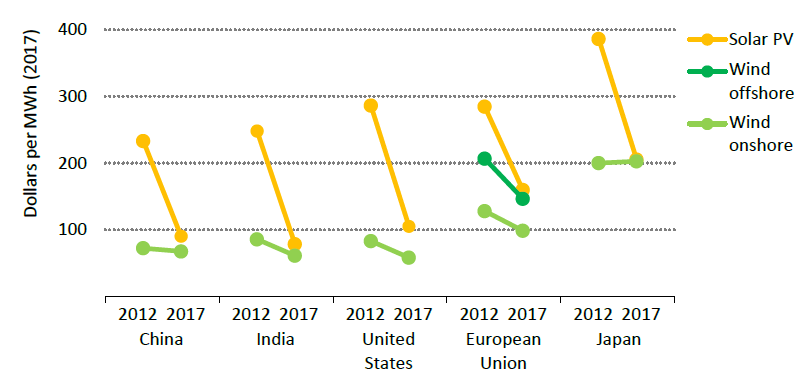
\includegraphics[width=10cm]{LCOE.PNG}
\caption[LCOE of Solar PV, Onshore wind and Offshore Wind]{LCOE of Solar PV, Onshore wind and Offshore Wind \cite{WEO}}
\label{Figure:1}
\end{figure}
\noindent
\newline 
\newline
To elaborate further on this projected price decrease, it is important to note that this capital cost evolution depends on how PV adoption will evolve over the next few decades. This evolution for different IEA scenarios can be seen in Figure \ref{Figure:adopt}.
\begin{figure}[h!]
\centering
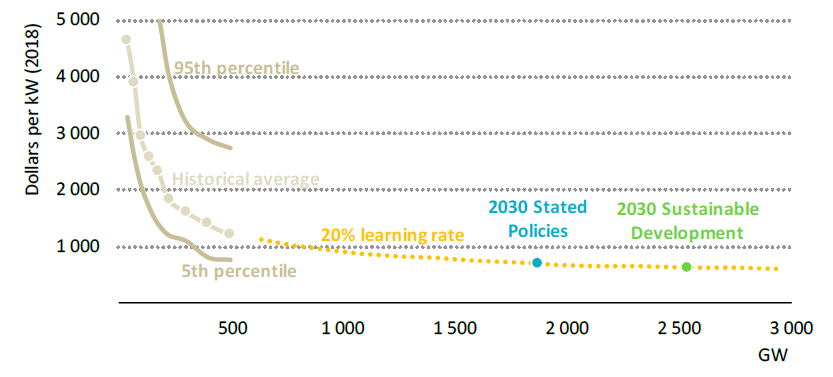
\includegraphics[width=10cm]{PVadoption.PNG}
\caption[Projection of PV capital cost]{Projection of PV capital cost \cite{WEO20}}
\label{Figure:adopt}
\end{figure}
\noindent
According to this Figure, the capital cost is set to decrease at a learning rate\footnote{The learning rate of a technology is the rate at which the cost will decrease if the cumulative installed capacity of the technology doubles} of 20\ . Depending on the adoption speed, therefore, the capital cost will decrease further. For both the Stated Policies and Sustainable Development, however, the capital cost is set to decrease significantly over the next few years. Since PV has no fuel costs, the capital cost decrease will have a major influence on the overall LCOE, which is also set to decrease further as time and adoption rates go by.  
 \newline \newline \noindent
% \textbf{Wind Power}
 %\newline \newline \noindent
 %Wind power, which is mainly exploited in the form of wind turbines, has become the most popular non-hydro renewable energy source in recent years. In 2018, 51.3GW of capacity was added, to bring the total wind power capacity to 591GW \cite{Wind18}. Like solar power, this adoption was initially fueled by government-backed incentives, followed by a decrease in price due to increased learning and scalability. As can be seen in Figure \ref{Figure:1}, the LCOE of onshore wind has seen a steady decrease (except in Japan) over the last few years. This LCOE is also expected to keep on decreasing, as can be seen in table \ref{table:1}.
%\begin{table}[h!]
%\begin{center}
 %\begin{tabular}{||c||c||c|c|c|c|c|c||} 
 %\hline
  %\multirow{\textbf{Region}} & \multirow{\textbf{Technology}} & \multicolumn{2}{c|}{\textbf{Capital} (\$/kW)} & \multicolumn{2}{c|}{\textbf{O\&M} (\$/MWh)} & \multicolumn{2}{c|}{\textbf{LCOE}     (\$/MWh)} \\  
   %\cline{3-8}
   %& & 2017 &2040 & 2017 & 2040 & 2017 & 2040\\
  %\hline 
%\multirow{USA}  & Nuclear & 5000 & 4500 & 30 & 30 & 105 & 100\\
 %&Coal & 2100 & 2100 & 30 & 35 & 75 & 75\\
 %&Gas CCGT & 1000 & 1000 & 30 & 40 & 50 & 65\\
%&Solar PV & 1560 & 860 & 10 & 5 & 105 & 50\\
 %&Wind onshore & 1620 & 1480 & 10 & 10 & 60 & 50\\
 %&Wind offshore & 4720 & 2960 & 40 & 25 & 180 & 105\\
%\hline
%\multirow{EU}  & Nuclear & 6600 & 4500 & 35 & 35 & 150 & 110\\
 %&Coal & 2000 & 2000 & 45 & 45 & 120 & 145\\
 %&Gas CCGT & 1000 & 1000 & 55 & 75 & 90 & 120\\
%&Solar PV & 1300 & 760 & 20 & 15 & 160 & 85\\
 %&Wind onshore & 1820 & 1700 & 20 & 15 & 100 & 90\\
 %&Wind offshore & 4260 & 2820 & 35 & 25 & 150 & 90\\
%\hline
%\multirow{China}  & Nuclear & 2320 & 2500 & 25 & 25 & 60 & 65\\
 %&Coal & 800 & 800 & 35 & 30 & 50 & 70\\
 %&Gas CCGT & 560 & 560 & 70 & 90 & 85 & 115\\
%&Solar PV & 1120 & 640 & 10 & 10 & 90 & 45\\
 %&Wind onshore & 1200 & 1180 & 15 & 15 & 70 & 65\\
 %&Wind offshore & 4120 & 2740 & 35 & 25 & 145 & 90\\
%\hline
%\multirow{India}  & Nuclear & 2800 & 2800 & 30 & 30 & 70 & 70\\
 %&Coal & 1200 & 1200 & 35 & 35 & 60 & 55\\
 %&Gas CCGT & 700 & 700 & 80 & 90 & 95 & 105\\
%&Solar PV & 1120 & 620 & 10 & 10 & 80 & 40\\
 %&Wind onshore & 1080 & 1040 & 10 & 10 & 60 & 50\\
 %&Wind offshore & 3320 & 2220 & 40 & 25 & 155 & 95\\
%\hline
%\end{tabular}
%\end{center}
%\caption[Overview of capital intensity of different technologies]{Overview of capital intensity of different technologies \cite{WEO}}
%\label{table:1}
%\end{table}
 %\newline 
% Despite the hype that exists around wind power, this technology has a few major issues. The first one is the fluctuations in the power output \cite{WindDisAd}. The second one, which is a result of the first one, is the sudden stresses wind power can cause on the grid stability \cite{WindStability}. When talking about wind power, however, one must make a distinction between onshore and offshore wind power, since both technologies do have some difference in costs, operation and regional popularity.
% \newline \newline \noindent
% Onshore wind has been deployed in most regions around the world. First developed in the 1980s, this technology gradually expanded through the 1990s to become a well-established technology. Over time, many countries started adopting wind power to make it achieve its state of popularity it enjoys now \cite{Onshoreoffshore}. Of the 51.3 GW that was installed in 2018, 46.8 GW was onshore (about 91.2\  of the overall installed capacity). The main advantages of onshore wind are its ease of installation, lower cost of installation and less maintenance difficulties. The disadvantages of the technology are its limited size potential, visual and auditive obstruction, and less constant wind patterns.
% \newline \newline \noindent
% Offshore wind is a smaller but very popular branch of wind power which is steadily increasing in capacity in Nothern Europe (note how data on offshore wind power is only available for the European Union in Figure \ref{Figure:1}). In 2018, only 8.8\  (or 4.5 GW) of all installed wind power capacity was offshore \cite{Onshoreoffshore}. Despite being more challenging to construct and maintain, the overall production and potential of offshore wind is higher than onshore and is so far underexploited.
% \newline \newline \noindent
% Due to its popularity, wind power has been severely decreasing in price over the last few years across all regions, as can be seen in Figure \ref{Figure:1}. This price is expected to decrease further in the future, as can be seen in table \ref{table:1}. In the EU, the capital cost for onshore wind power is projected to decrease from $1820\frac{\$}{kW}$ in 2017 to $1700\frac{\$}{kW}$ in 2040, a 6.6\  decrease, while offshore wind power is projected to decrease from $4260\frac{\$}{kW}$ in 2017 to $2820\frac{\$}{kW}$ in 2040, which is a decrease of 33.8\ 
% Fueled by this popularity, the amount of wind power capacity is expected to triple by 2040, as can be seen in Figure \ref{Figure:global}. Some even claim this technology has sufficient potential to meet the worlds entire electricity demand if well managed \cite{WindPotential}. Fueled by continuously decreasing costs (up to 40\  by 2050), the technology is often called a 'game-changer' in the electricity generation transition.
% %\newline \newline \newline \noindent
%\newline \newline \noindent
\textbf{Residential Batteries}
\newline \newline \noindent
The need for residential storage is becoming a major concern for the efficient implementation of DERs in a residential context because of the intermittent character of renewable energy technologies. Due to the mismatch between PV production and residential consumption patterns, storage is an important means to reduce the destabilizing grid injection of residential PV during peak production and low consumption. The amount of storage capacity on a global level, however, is very low compared to the overall production capacity, as can be seen in Figure \ref{Figure:storage}. The overall storage capacity was 2.2\  of the total generation capacity. Of this overall capacity, however, the vast majority of the storage infrastructure is pumped hydro storage (98.9\  of the overall storage capacity is in pumped hydro storage). Only a portion of the remaining storage capacity is battery storage. The overall battery storage capacity has historically, therefore, been very low. 
\newline
\begin{figure}[h!]
\centering
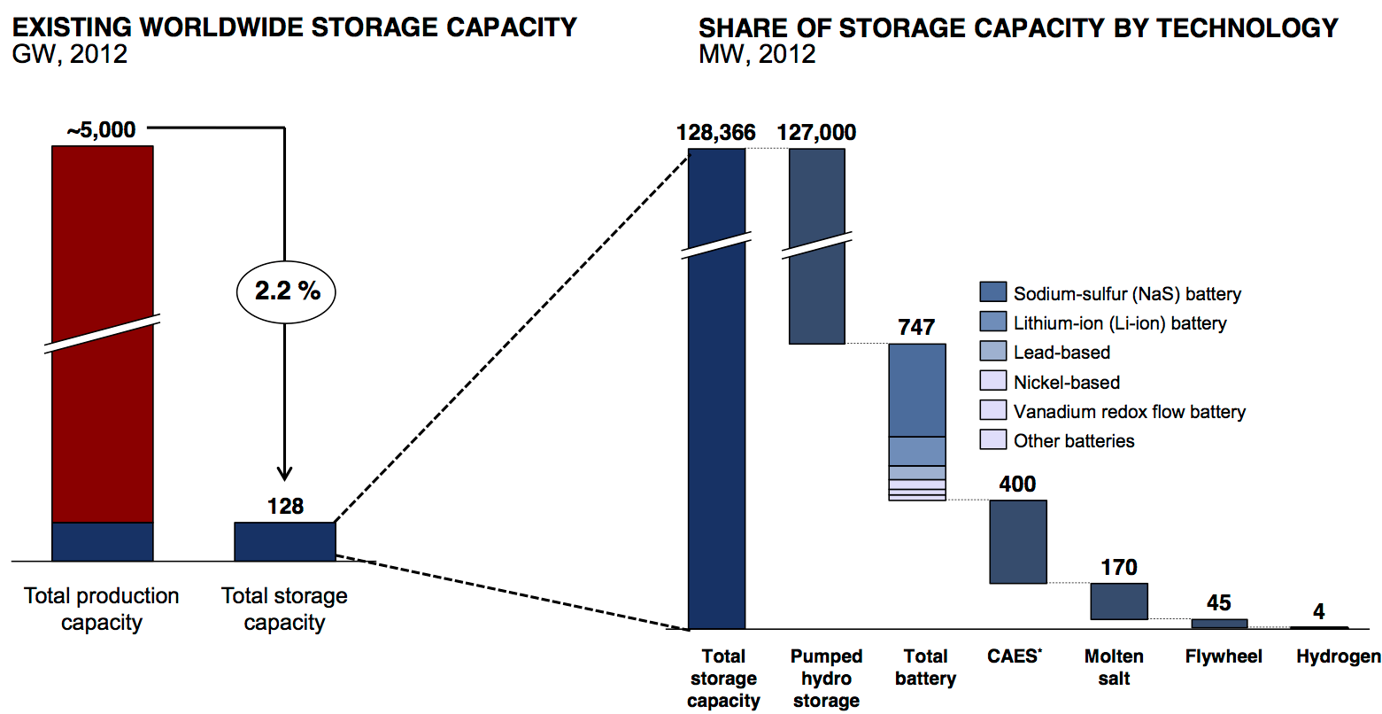
\includegraphics[width=10cm]{Storage.png}
\caption[Global storage capacity]{Global storage capacity \cite{Storage}}
\label{Figure:storage}
\end{figure}
\noindent
\newline
Even though the overall storage capacity in the world is very low and battery storage accounts for an even smaller portion of the overall storage capacity, storage capacity has been increasing rapidly, at a CAGR of 73\  between 2013 and 2018 \cite{Storage}. This large growth, however, will make the most recent values of the overall battery storage capacity (3.1 GW) still account for only a small portion of the global generation capacity. When comparing this value with the most recent data available for the global power generation capacity, which is a value of 7220 GW, it becomes clear the proportion between these two values is very unbalanced (the global generation capacity outnumber the battery storage capacity by a factor of 2329). 
\newline \newline \noindent
Since storage is often postulated as a major solution to the intermittent and unpredictable production patterns of wind and solar electricity generation, it may be interesting to consider what level of storage is required to allow for high renewables penetration in the grid. Solomon et al. tried to address this question by examining different cases of high renewables integration \cite{penetration}. In this research, the minimal amount of battery storage capacity required for a 90\  renewables penetration was determined to be the equivalent of the daily demand for electricity. To ensure minimal power loss, this storage capacity should be even higher. To ensure a reliable grid integration with large amounts of intermittent generation (i.e. large amount of solar and wind power, as is projected in Figure \ref{Figure:global}), the amount of storage will have to drastically increase over the next few decades. This increase require increased investments in residential battery systems, like Tesla Powerwall. Nevertheless, the emergence of electric vehicles (EV) can partially offset the need for investments in stationary storage capacity since EV batteries can also be used for residential storage purposes \cite{EV1,EV2}. 
\newline \newline \noindent
Despite being quite expensive nowadays, battery technology prices are expected to decrease rapidly over the next few years. Lithium-ion batteries, to take an example\footnote{In recent years, this technology has become the most promising battery technology, mainly due to its usage in Tesla and other electric automobiles}, have seen its levelised cost of storage (LCOS) decrease from \$1,160 in 2010 to \$176 in 2018, as can be seen in Figure \ref{Figure:bloom}.
\newline 
\begin{figure}[h!]
\centering
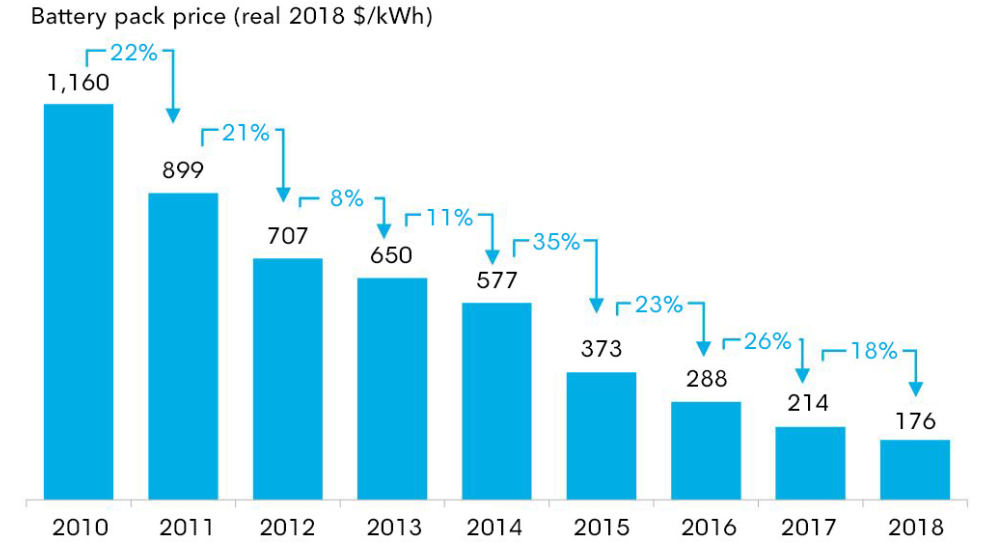
\includegraphics[width=10cm]{LCOS.PNG}
\caption[LCOS of Lithium-ion]{LCOS of Lithium-ion \cite{bloomberg}}
\label{Figure:bloom}
\end{figure}
\newline 
This LCOS is expected to decrease further to 94 $\frac{\$}{kWh}$ in 2024 and 62 $\frac{\$}{kWh}$ in 2030 \cite{bloomberg}. This projected decrease in price, combined with the increasing demand for batteries for grid integration purposes, will cause battery adoption to increase significantly over the next few decades, as can be seen in Figure \ref{Figure:global}.
\newline \newline \noindent
\textbf{Other}
\newline \newline \noindent
Although there are many more emerging technologies that can be implemented in a distributed context, these go beyond the scope of this Thesis. A quick enumeration of these technologies, however, will still be done. Wind power, both onshore and offshore, is the most prominent one. Another one is geothermal heat on a residential level, where ground heat is used for passive cooling and heating on a residential level. In this Thesis, electrical storage is considered, but thermal storage is also a form of DERs that is gaining popularity. Other forms of DERs include small hydro, biomass, biogas and small wind turbines.

%\subsection{DERs investment data}
%Having discussed which technologies are shaping the future electricity system, an overview of investments and capacity additions of these technologies will be discussed. According to the International Energy Agency, worldwide investments in electricity generation, networks and storage amounted \$750 billion in 2017 \cite{WEO}. Of the overall investment amount in electricity generation assets, two-thirds went to renewable assets. Figure \ref{Figure:RESINV} shows how these investments in different renewable energy technologies have evolved in the period 2013-2017.
%\begin{figure}[h!]
%\centering
%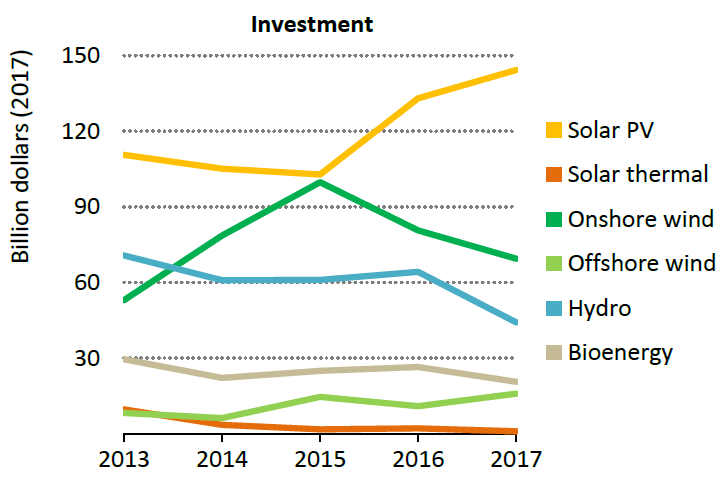
\includegraphics[width=8cm]{RESinvest.PNG}
%\caption[Global investments in renewable electricity investments]{Capacity for energy transition \cite{WEO}}
%\label{Figure:RESINV}
%\end{figure}
%\noindent
%\newline
%Judging by the evolution of the different curves in this Figure, solar PV is the most popular technology among investors in recent years. Surprisingly, investments in onshore wind decreased in the period '15-'17 after a period of growth in '13-'15. The investments in offshore wind, on the other hand, increased. The capacity additions that result from the investment data in Figure \ref{Figure:RESINV} can be found in Figure \ref{Figure:CAP}.
%\newline
%\begin{figure}[h!]
%\centering
%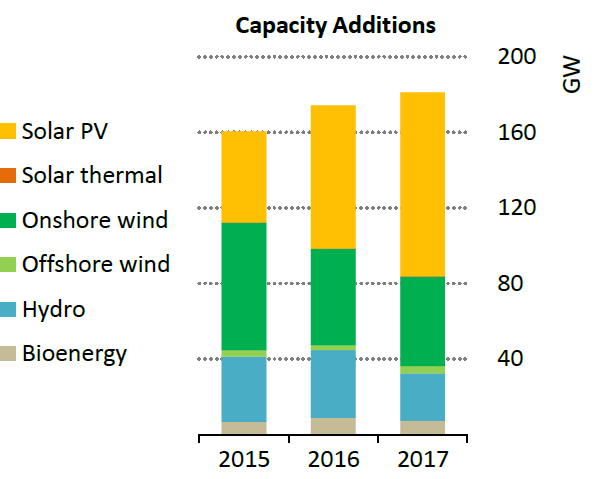
\includegraphics[width=8cm]{REScap.PNG}
%\caption[Global RES capacity additions]{Global RES capacity additions \cite{WEO}}
%\label{Figure:CAP}
%\end{figure}
%\noindent
%\newline 
%As is the case with the investment data, solar PV additions have been dominating the overall RES capacity additions in the period 2013-2017. When considering how these additions compare to the addition of fossil fuel electricity generation technologies like oil-fueled plants, coal-fired power plants, or CCGT, Figure \ref{Figure:comparions} shows that the amount of RES capacity added in 2017 surpasses the amount of conventional, fossil fuel capacity added in that period. This clearly shows how DERs, especially solar PV, are gaining popularity and will shape the future of the electricity market.
%\newline 
%\begin{figure}[h!]
%\centering
%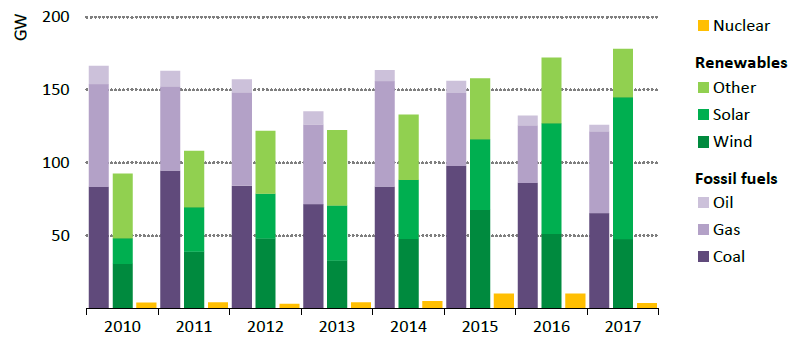
\includegraphics[width=10cm]{comparison.PNG}
%\caption[Global RES and fossil fuel capacity additions]{Global RES and fossil fuel capacity additions  \cite{WEO}}
%\label{Figure:comparions}
%\end{figure}
%\newline
%When looking into the future, the extent of the additional investments required in DERs and other renewables is also an interesting consideration. Since the call for a massive reduction of emissions is becomes more and more clear, there has been research into what the investment requirements are to meet a near-to-zero emission energy infrastructure over the next three decades, as was done by Jacobson et al. \cite{jacobson}. In this work, the cost of the New Green Deal to transition to a 100\  clean energy system was evaluated. This new infrastructure, consisting of wind, water and solar energy, increased efficiency and storage technology, is estimated to come at a cost of \$73 trillion if the objectives are to be met by 2050. The International Energy Agency estimates the cost of performing the New Policies Scenario and Sustainable Development Scenario at \$60 trillion and \$68 trillion, respectively, as can be seen in Figure  \ref{Figure:transition}. 
%\newline
%\begin{figure}[h!]
%\centering
%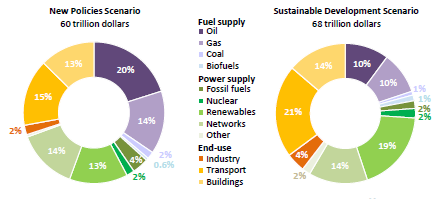
\includegraphics[width=\textwidth]{scenarioInvestment.PNG}
%\caption[Investment overview for IEA Scenarios]{Investment overview for IEA Scenarios \cite{WEO}}
%\label{Figure:transition}
%\end{figure}
%\noindent
%\newline
%Note how in both these scenarios, the investments in power supply are a substantial part of the total investments. For the New Policies Scenarios, the projected investments in renewable power supply technologies amount to 13\  of the total investment, or\$7.8 trillion, while for the Sustainable Development Scenario the portion for renewables is 19\ , or \$12.92 trillion. Although this is a sizeable investment amount for both scenarios, over time these goals must be met to ensure a sustainable energy infrastructure in the future.
\section{Investments in Distributed Energy Resources} \label{Investmentss}   
\subsection{Introduction}
In this section, the drivers, characteristics, and consequences of investments in DERs will be discussed. First of all, the characteristics of DERs investments will be discussed. This discussion will subsequently be narrowed to investments in PV and the resulting adoption patterns that arise from these investments. To conclude, a few points of attention in the investment in DERs and PVs, in particular, will be discussed.
% \subsection{DERs Investment Characteristics}
% When considering the installation of a PV-battery or another DERs, one must actually consider if this infrastructure expense is an investment altogether, since the costs a household must incur for a PV-battery installation is of the same magnitude as certain consumption goods\footnote{The investment in a PV-battery system, as will become clear in Chapter 3, is of the magnitude \$5,000 - \$10,000. Compared to certain household consumption appliances like electronics or transportation, this is a comparable cost}. An expense in a certain asset can be classified as an infrastructure investment if the following criteria are met \cite{infrastructure}:
% \begin{itemize}
%     \item \textbf{Asset exposure}: The infrastructure that is invested in consists of tangible assets.
%     \item \textbf{Stable, inflation-linked cash flows}: The infrastructure asset must generate a certain cash  flow that benefits the %investor throughout its operational lifetime.
%     \item \textbf{Long asset life:} The definition of a 'long lifetime' in this case refers to a value of  twenty years or longer. 
 %    \item \textbf{Uncorrelated to the equity markets, GDP and systemic risk}: The performance of the asset must  not be dependent on financial markets, as equities and fixed income do. This can either be for better or for  worse: the systemic risk of a financial collapse cannot directly influence the performance of the infrastructure asset.
     %\item \textbf{Direct investment can lead to low fees due to low maintenance costs}: The majority (or at least a large part) of the overall cost is in the capital investment into the asset.
 %\end{itemize}
 %When considering how an investment in a DERs like a PV-battery installation fits into these characteristics, there are a lot of similarities to be spotted. A PV-battery system is a tangible object. Since a PV-battery will cause the household to consume less electricity from the grid, the electricity bill for the household will be lower than it would have been if the household had not installed a PV-battery system. The cash flows the installation will generate are the savings caused in electricity cost due to lower gird offtake. Even though electricity prices tend to vary and are not inflation-linked, the cash flows that will be generated by this installation are going to be reasonably stable. 
% \newline \newline \noindent
 %The operational energy lifetime of a PV module is currently estimated about 20 to 25 years \cite{lifetime,lifetime2}. Given certain further innovations, this lifetime could increase to as much as 50 years \cite{lifetime3}. Throughout this lifetime, the cash flows will steadily be generated.
% Since the cash flow mainly depends on the electricity price, the effect of the financial markets and GDP is very limited in this cash flow generation. This electricity price is quite heavily regulated and will, therefore, not be completely exposed to the systemic risk of the equity and other financial markets. Finally, to comment on the last criterion, the maintenance and other operational costs of the PV-battery system are low, since there are no fuel costs.
 %\newline \newline 
% \noindent
 %The installation of a PV-battery system, therefore, clearly is an infrastructure investment. When considering what the actual characteristics of this DERs are, a few points must be commented upon. Olsina et al. listed several characteristics of power generation investments \cite{3}. Although this work concerns investments in power plants, these characteristics also apply to DERs investments. These include capital intensity, sunk cost, one-step investment, long-run uncertainties, long payback periods, investment irreversibility and investment postponement options.  
% \subsubsection{Capital intensity}
 %Although the investment in residential PV-battery systems is a limited financial commitment, this investment only accounts for a limited amount of production capacity. To get an idea of the overall capital requirements of DERs, table \ref{table:1} gives an overview of the cost components for different electricity generation technologies. Looking at the data in this table, it becomes clear that the capital cost of the renewable DERs still is higher than some conventional technologies. Solar PV still has higher capital requirements than gas CCGT in most regions, whereas offshore wind still is more expensive than coal-fired plants and gas CCGT. The second trend that can be noted, as has been discussed in section \ref{Trends}, is that the capital costs of renewable DERs like solar PV and wind power are set to decline significantly over the next few decades. 
% \newline \newline \noindent
 %Investing in DERs like solar PV and wind power, therefore, is a capital intensive process. To illustrate this, the data in table \ref{table:cost} shows the estimated capital requirement for different generation capacities. As can be seen, the total investment amount for an industrial-scale generation plant like Doel Power Station is very high, because of high capital cost and a high power plant capacity. The investment amount for a residential PV installation, on the other hand, is much lower because the capacity is much lower. 
 %\newline 
 %\begin{table}[h!]
 %\begin{center}
 % \begin{tabular}{||c|c|c|c||} 
 % \hline 
  %\textbf{Power plant} & \textbf{Technology} & \textbf{Capacity }(MW) & \textbf{Capital cost} (\$)\\
  %\hline
  %Doel power plant & Nuclear (PWR) & 2,923 & 19,291,800,000 \\
  %Ibbenbüren power plant & Coal-fired & 838 & 1,676,000,000\\
  %Amercoeur Power Unit & CCGT & 420 & 420,000,000\\ 
  %Vestas Wind Turbine & Onshore Wind & 4 & 7,644,00 0\\
 %PV installation & Solar PV & 0.004 & 5,200\ \
 % \hline
 %PV installation & Solar PV & 2,923 & 3,799,900,000\\
 % \hline
 % \end{tabular}
 % \end{center}
 % \caption[Nameplate capacity \& estimated capital cost of different]{Nameplate capacity \& estimated capital  cost of different %\cite{Vestas,Doel,Ibbenburen,Amercoeur}}
  %\label{table:cost}
 %\end{table}
 %\noindent
 %\newline 
 %When considering what the total investment in solar PV would be to obtain the same capacity as a large power generation station like Doel, it becomes clear that this amount is also considerable. Considering the load factor of PV panels is much lower than that of a power plant like a PWR or CCGT, the amount of capacity required for the same amount of energy produced will be much higher, thereby increasing the investment requirement even more. 
 %\subsubsection{Long-run uncertainties}
 %The combination of large investments, long lifetimes, and long payback periods pose a significant risk to the economic viability of DERs. A large number of possible risks exist, which can negatively influence the economics of the DERs. A few important ones are:
 %\begin{itemize}
 %    \item \textbf{Weather conditions}: Although not very important for fossil fuel power plants, this factor is very important for the emerging renewable technologies like wind and solar PV, since the performance of these technologies directly depends on the governing  weather conditions. Note that this uncertainty is predominantly short-run, since weather conditions can rapidly change, but also long-run to a certain extent due to changing weather patterns over the last few decades, as has been examined in Pakistan and the Himalayas \cite{Weather} and many more places around the world.
 %  \item \textbf{Future demand}: Depending on the future demand for electricity, the DER in construction or operation may not even be necessary at a certain point in the future. The fact that the generation capacity may potentially become obsolete in the future provides an additional level of uncertainty to the investment.
 %  \item \textbf{Long-term electricity prices}: The long term change in electricity prices can have a severe influence on the economics of any electricity generation asset. Since the economics of DERs depend on the potential savings they can realize, electricity prices are an important factor in assessing the economics of adopting a DER. If the electricity prices were to steadily increase over time, on-site production would become more attractive since the savings realized by the DER are going to increase, but if the electricity prices will decrease over time, the on-site production will become less attractive since the savings realized by the DER are going to decrease. 
 %\end{itemize}
 %Other parameters that need to be accounted for include:
 %\begin{itemize}
  % \item \textbf{Technological innovation}: The entry of more efficient technologies into the electricity generation landscape could easily substitute an existing technology, thereby making existing power plants or DERs unpopular. In the context of emerging small-scale technology, this is quite a big risk since the emergence of a technology could easily be hampered by another technology.
  % \item \textbf{Policy changes}: Since liberal electricity markets are relatively young, there is a continuous process of changing policies, which can influence the attractiveness of a certain generation technology. Especially for DERs, with government incentives like green certificates and Feed-in Tariffs (FiT) being regular topics of debate, these policy changes can pose a risk to the attractiveness of certain DERs. 
 %\end{itemize}
 %\subsubsection{Large sunk cost}
 %\noindent
 %Besides demanding large capital commitments, investments in DERs will also have what is called a sunk cost. This sunk cost, which is not only the case for electricity investments but any kind of dedicated infrastructure investment, is a cost that has already been incurred but that cannot be recovered. In the case of the electricity sector, a firm or another investor could incur a sunk cost if a certain power generation asset cannot be sold or transformed for another purpose without too much effort.
 %\newline \newline \noindent
 %In the current context of emerging technologies, conventional technologies with a long lead time and lifetime face an additional challenge. Throughout the lifetime of a certain electricity generation asset, technical progress comes in to play. The sudden emergence of a new energy technology could make certain DERs in use economically unattractive, forcing the investor to incur large costs \cite{Helm}.
 %\newline \newline \noindent
 %Although the absolute investment requirement for renewable energy technologies is lower, as was illustrated in table \ref{table:cost}, these technologies also have a very high sunk cost, proportionally even higher than is the case for conventional power plants. Renewable energy technologies like solar or wind do not have any fuel costs, contrary to conventional power generation. The majority of the costs in the technology, therefore, will be in the investment in the technology itself.
 %The sunk cost can, therefore, account for a very large proportion of the overall costs for DERs, posing a significant risk to the investor.
 %\subsubsection{One-step investment}
 %When installing a DER installation, a lot of functionalities must be fulfilled to make the unit operational. Therefore, a large amount of capital expenditures is required before the production capacity can become operational. Once this capacity is operational, the required capex required is merely maintenance capex and will, therefore, account for a limited amount of the overall capital requirements. 
% \subsubsection{Long payback period}
% The combination of a high overall cost and a large one-step investment for electricity generation assets will demand a high financial commitment by the investor, which often will be partially financed with debt. Over the duration of the operational lifetime, therefore, this debt will have to reimbursed. Considering the fact that the lifetime of a PV installation is about 20 years and 25 years for a wind turbine, the payback period for these assets can easily be years. There has been a some research in these matters \cite{Czec,CSP}. In \cite{Czec}, the payback period of a photovoltaic power plant was studied back in 2010, which came to 10-11 years, almost half the overall lifetime of the technology. In \cite{CSP}, the payback period of concentrated solar plant (CSP) was calculated, with results that go from 3.5 to 6 years, also a significant portion of the lifetime of a CSP plant. The overall payback period for DERs, therefore, is significant for different renewable energy technologies.
% \subsubsection{Investment irreversibility}
% The investment in generation capacity is considered a form of sunk cost, since a power plant can only serve the purpose it is designed for. If market conditions turn unfavorable and render the power plant unprofitable, there is little other purpose that the power plant infrastructure can serve. Even if it were to be sold, it would probably have to be done so at a loss. 
% There has been related work describing the irreversibility of investments in power generation \cite{irreversible}.
% \subsubsection{Investment postponement option}
% Since investing in a power plant or DER requires some financial commitment on behalf of the investor, it is very easy for the investing party to decide to postpone this decision. Especially in the context of investing in small-scale renewable technologies, where policies, tariffs and subsidies tend to change regularly, potential investors could easily choose to await new subsidies or tariffs before deciding to invest in DERs. In the case of DERs, there also is no immediate urgency for the technology to be installed, since electricity will remain available from the grid, which only adds to the possibility to postpone the investment. 
 \subsection{PV characteristics}
 \newline \newline \noindent 
 With the knowledge of the general investment characteristics of DERs, the scope can be narrowed to the technology that is under consideration in this Thesis, being solar PV. For the specific case of PV technology, there are a few specific investment characteristics that can be identified and can make it a preferred choice over solar powers greatest competitor, wind power. These can be grouped into three categories, as was identified by Ernst\&Young: operational, scalability and financial \cite{EY}.
 \subsubsection{Operational}
 There are a few potentials costs and benefits to investors because of technical characteristics of solar power. First of all, there will be less inherent production uncertainty, since solar irradiation forecast usually are more reliable than wind forecast. The increased reliability of the forecasts makes the future production of solar PV more certain, thereby making the future cash flows more certain, which makes the investment in solar PV more attractive compared to other intermittent DERs.
 \newline \newline \noindent
 In addition, the technology risk is lower compared to wind power due to less moving parts and few mechanical parts. Since residential PVs are installed on the roof of any residence, maintenance is very easy due to the accessibility of the installation. Compared to wind turbines (especially offshore), therefore, maintenance cost are much lower. Due to this major accessibility and fewer mechanical/moving parts, the lead time of a PV project, even a big one, is limited to months, compared to years for some large wind projects. 
 \subsubsection{Scalability}
 In addition to having interesting operational advantages, solar power has interesting scalability characteristics due its modularity. First of all, since solar panels can be fitted on any surface, flat or inclined at an angle, solar panels can be fitted anywhere. This makes it easy to install solar close to where the demand is, closer than any other renewable DER. Since the smallest unit size also is so small, the design of PV configurations is very modular and can range from kWs to MWs. Depending on the available space for installing solar PV modules, the number of modules can be adapted. Solar PV, therefore, is a very flexible technology in terms of installation and size, making it appeal to a wide range of investors, more than other DERs. 
 \subsubsection{Financial}
 As a final advantage, solar panels can also be a good investment for someone seeking returns on his or her investment. Ernst \& Young estimates that over the course of the next 35 years, the expected annual returns generated by investments in solar panels can vary anywhere between 6.6\  and 10.1\ , depending on how the efforts to combat climate change evolve \cite{mercer}. To put this into perspective, a US government bond will yield an annual return between 0.03\  and 1.30\ , depending on the maturity of the bond \cite{bonds}. The benchmark for the stock market, the S\&P 500, has had an average annual return of 9.8\  over the last 90 years \cite{stocks}. The returns of the solar panels, therefore, make a strong case for investments in because of good returns on investment.
 \subsection{Investment Drivers}
 As with many emerging trends, there are several drivers behind the emergence of small-scale renewables. These drivers cut across technical, economic, and environmental dimensions. Due to the increasing levels of pollution on a global level and the increasing awareness that this pollution might have dire consequences for the planet, there are strong environmental arguments for the rapid adoption of small-scale renewable DERs
 \newline \newline \noindent
 Since DERs will provide on-site production and storage of electricity, their adoption could have several technical advantages. First of all, since the DERs do not depend on the transmission or distribution grid for electricity production, remote communities can rely on these DERs to be self-sufficient in their electricity needs. In addition, grid operators will not need to extend their costly infrastructure to these remote areas to serve just a few customers. DERs, therefore, could avoid a great deal of expenses for the grid operators while making these remote communities self-sufficient. The case for the synergies that can be created by adoption DERs in remote areas has been made in numerous works for remote areas in Western Australia, Alaska and Canada \cite{remote1,remote2,remote3}. All this research strongly supports remote DERs adoption, provided that sufficient storage capacity is installed, to mitigate the risk of power shortages.
 \newline \newline \noindent
 In areas where there is a transmission and distribution infrastructure, DERs can help reinforcing the grid resilience by improving grid balancing. The importance of distributed resources for balancing purposes has been studied in other work \cite{balancing}. In this work, the authors were able to show that local storage devices are preferable compared to a central capacity. The authors in \cite{balancing2} also showed the usefulness of having local DERs assets for increased flexibility and balancing possibilities. In addition to these technical advantage associated with DERs, some other advantages have been identified \cite{technical}.  
 \newline \newline \noindent
 First of all, the DERs reduce the cost of energy, since the grid infrastructure doesn't have to be extended to all possible consumers if DERs can be adopted. Since more people can have access to electricity (and also heat and cooling when cogeneration is being used) by adopting DERs, the overall security of supply of the power system increases. Since production becomes more on-site and self-sufficient through DERs adoption, the reliability of the power system increases (since supply no longer depends on a central producer but many remote and local producers), which will make the consequences of a power outage on the grid less severe and costly. Since many of the DERs are renewable energy technologies, like solar PV, wind power and biomass, the adoption of DERs will go in parallel with a reduction of greenhouse gas emissions. Since more of the demand will be met by on-site production, there is also less need for constructing large generation units, relaxing the investment requirements for large utility providers. In the case of renewable DERs that don't require any fuel for operation, the fuel dependency, fuel cost risk and fuel supply will decrease for larger communities. Ancillary services can also be provided by DERs.  As a final point, DERs can increase the energy efficiency levels of the overall energy infrastructure. 
 \newline \newline \noindent
 Note how the three main pillars of sustainability, being security of supply, affordability and reduced pollution, all fit in the adoption of DERs. This is one of the reasons why this class of energy technologies is so promising for the future energy infrastructure.  
\subsection{Adoption of DERs on a household level}
Having discussed the characteristics and drivers of the investments in DERs, PV in particular, some empirical data on the adoption of DERs can be discussed. Since the focus in this Thesis is on the household level, it is important to determine    what the evolution of PV has been on a residential level and what the main drivers of this adoption are. There has been research into the diffusion of residential PV in different regions, such as Flanders \cite{FlandersAdoption} and Italy \cite{ItalyAdoption}. In addition there has been research into the evaluation of different policies related to PV technology and their effect on the evolution of PV adoption \cite{ABMPV}. 
\newline \newline \noindent
It may be interesting, at this point, to identify the main drivers of residential PV adoption, since this will provide insights for the model development in Chapter 3. In \cite{FlandersAdoption}, these drivers are identified. Since this work considers the drivers of Flanders, where the KU Leuven is located, an extensive discussion of these drivers is appropriate. The main drivers were identified to be: 
\begin{itemize}
    \item \textbf{Local subsidies}: These incentives, as there are green certificates and net metering, have had a significant impact on the adoption of PV technology in Flanders, especially when the cost of this technology was significantly higher in the recent past. Additionally, the more regional subsidies and incentives also seem to have benefited the evolution of the PV adoption rates.
    \item \textbf{Dispersion of income}: Through these subsidies, it was found that mostly rich households were able to benefit from these subsidies. The average income and economic status of the household adoption the PV, therefore, is also an important driver of PV adoption. 
    \item \textbf{Value of a house/household size}: With respect to the previous driver of PV adoption, it should be noted that an additional driver for PV adoption is the household size and house ownership. Since a larger family will, on average, consume more electricity, the incentive for PV adoption will be higher. On average, larger households will also have houses that are more conducive to the installation of PV technology, thereby increases adoption in this household category. If a certain households is the owner of a house, the decision power lies only with the occupant of the house, since he is the owner as well. This will make PV adoption more likely in this household category. If,on the other hand, the household is renting the house, the decision power lies with an external party, making the adoption of PV less likely.
    \item \textbf{Household characteristics}: A final aspect that will determine PV adoption is the 'characteristic' of the household, most importantly the age and size of the house. Overall, PV adoption is more likely in large or recently built houses. Since younger families will, on average, live in more recently built homes, this age category will have a larger percentage of PV adoption.  Despite this possibly being a result of changing mores between generations, the authors in \cite{FlandersAdoption} argue that this mainly is due to the fact that younger families will live in younger houses, not the actual age of the family.  
\end{itemize}
To elaborate on a few of these items, Palmer et al. showed that the economic profitability of the investment (through decreasing prices and subsidies) is the largest driver for adoption. In addition, the adoption will be the most stimulated by a gradual withdrawal of supportive measures, rather than abruptly withdrawing these \cite{ItalyAdoption}. As is the case in this Thesis, the authors consider different drivers than merely the economic ones, like the environmental and communication aspect in new technology adoption. The weight of these non-economic decision factors is lower than the economic weight. Their influence is also of limited duration. Over the longer term, the popularity of the PV technology will depend on the economic viability of this technology. De Villena et al. studied how different regulatory frameworks and incentive schemes by the government could influence the economic attractiveness of certain DERs \cite{Regulation}. To incentivize the DERs adoption, volumetric distribution rates rather than fixed ones should be implemented. The authors also determined net billing to be a better alternative than net metering to minimize the effects of the utility death spiral in the grid (see section \ref{spiral}). This work, however, assumes full rationality of the agents. Robinson and Rai use bounded rationality to determine factors influencing energy technology adoption \cite{spatiotemp,spatiotemp2}. An interesting finding in their work is the required incentives for PV adoption in lower-income. To have a significant impact on the adoption levels among low-income household, the rebates/incentives in PV cost must be substantial. Another interesting finding is in the time dependency of the rebate levels. If rebate levels are changed early in a program, when the amount of adopters is limited, the effect on the technology adoption is limited. If this rebate level is changed in a later stage of adoption, when the number of adopters is much larger, the effects will be more visible, since the social effect between adopters will cause the adoption to change. Zhao et al. argue that besides the household profile and the payback period of the PV, there are other factors at play \cite{ABMPV}. These mainly include the advertisement effect and the neighborhood effects. These two effects will account for the human perception of the product. In this Thesis, this will be represented as social utility (see Chapter 3\&4). From a technical point of view, Murakami combined the analysis of electric power flows from residential PV and social effects to determine how social policy and neighboring effects influence the diffusion of residential PV configurations \cite{flowanalysis}. The research points at that government intervention with regards to reverse current in the grid due to grid injection by peak PV production during periods of low demand, can have significant effects on the PV technology diffusion. By limiting the permitted reverse current, especially close to high-power distribution transformers, the diffusion is further enhanced. This will cause less variations in the voltage levels in the grid, reducing fluctuations and the need for batteries, which reduces to overall cost of DERs adoption. In areas located further from the distribution transformers, this reverse restriction must be relaxed since the overall system cost will increase due to higher requirements in battery capacity. The batteries are necessary to compensate for the lost possibility to inject power into the grid, causing the overall system cost to increase.
\newline \newline \noindent
When taking a step back from the adoption drivers and considering the adoption data itself, it becomes clear that PV is undergoing a rapid growth trend, as has been discussed in Chapter 1. The CAGR of the PV capacity (36.9 \  between 2010 and 2018) shows to what extent the global PV capacity has been growing. The future evolution of PV capacity can be found in Figure \ref{Figure:PVfut}. When focusing a bit more on the exact split between the different kinds of configurations installed, Figure \ref{Figure:split} shows that for the case of Italy, most of the installed PV installations in 2010-2011 had capacities between 1 and 20 kW, which is a size that can be implemented on a residential level.
\newline 
\begin{figure}[h!]
\centering
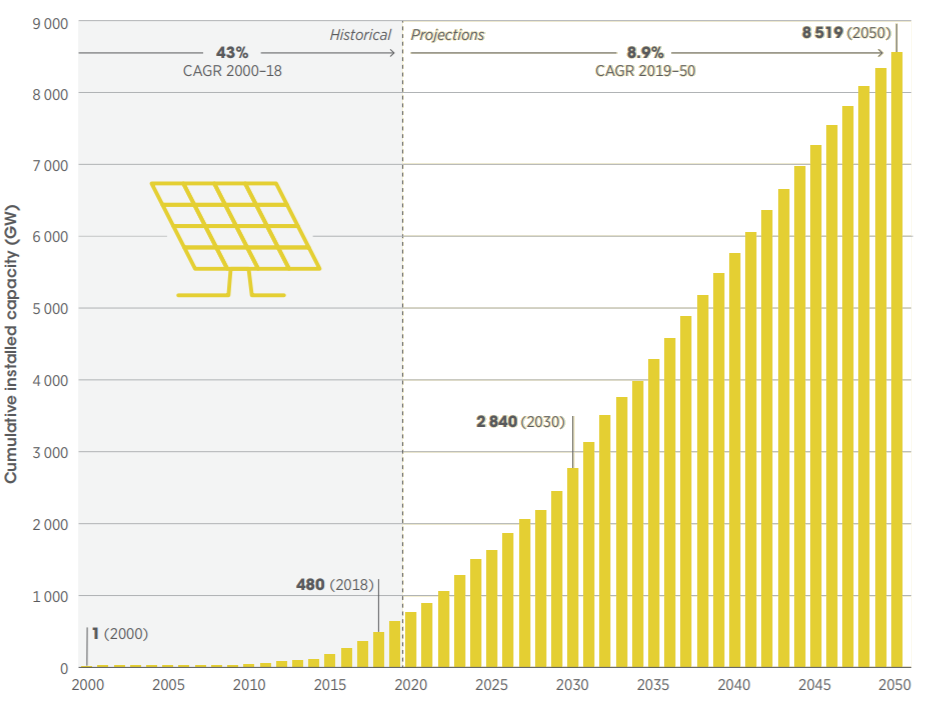
\includegraphics[width=6m]{PVfuture.png}
\caption[PV capacity evolution]{PV capacity evolution \cite{PVevolution}}
\label{Figure:PVfut}
\end{figure} 

\newline 
\begin{figure}[h!]
\centering
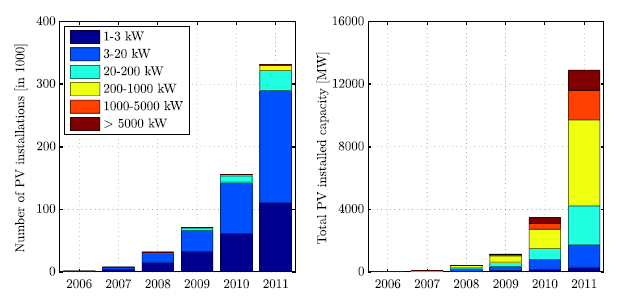
\includegraphics[width=10cm]{PVsplit.PNG}
\caption[PV configuration split]{PV configuration split \cite{ItalyAdoption}}
\label{Figure:split}
\end{figure}
\newline 
When looking at the overall capacity, however, it seems that the majority of the installations are in the range of 200 kW - 1MW. These installations, which may appear on large buildings or industrial estates, are also an important part of the overall PV adoption Figures. The adoption of PV on a residential level, therefore, is a consequence of various socio-economic factors. While social and other circumstantial factors play an important role in explaining adoption on a residential level, the economic consideration in the investment decision process remains the most important one.
 \subsection{Potential drawbacks}
 Over the course of the last few sections, the potential benefits and drivers for the adoption of small-scale DERs have been discussed. There are, however, also a few potential drawback or risks of this large scale DERs adoption. These include large area requirements, intermittency, grid requirements, material usage and, finally, the utility death spiral. Since the latter is an important phenomenon in the scope of this Thesis, it will be discussed separately in the next section. The other items, being very important to the overall DERs adoption discussion but less relevant in this dissertation, will be briefly discussed over the next few paragraphs.
 \newline \newline \noindent
 As has been discussed in the previous section, DERs technologies like PV and wind power are going to become increasingly popular (see Figure \ref{Figure:global}). These intermittent electricity generation sources add a level of uncertainty and complexity to the grid, since the supply and demand patterns of a renewable electricity production market will rarely align. As was discussed in section \ref{Trends}, there will be an increasing demand for storage capacity to cover this discrepancy between supply and demand patterns. In addition, the grid itself will need updates, to make its functioning more flexible and allow all DERs to be integrate into the functioning of the grid. The solution for this increased flexibility is not straightforward, since there still is debate on both sides of the argument whether the solution is a smart grid or super grid \cite{integration2} and how emerging technologies like EVs will be integrated into this grid \cite{integration1}. 
 \newline \newline \noindent
 In addition to imposing strict requirements on the entire grid, DERs will require a fair amount of land area to be able to meet the sustainability goals in the future. In a study by Cheng and Hammond, the energy density (in $\frac{GWh}{km^2}$) was determined for a few different energy generation technologies \cite{land}. A glossary of the data can be found in table \ref{table:land}
 \noindent 
 \begin{table}[h!]
 \begin{center}
  \begin{tabular}{||c|c||} 
  \hline 
  \textbf{Technology} & \textbf{Land density $(\frac{GWh}{km^2})$}\\
  \hline
  Nuclear (diffusion) & 3233 \\
  %uclear (centrifuge) & 3371\\
  Wind onshore & 872.4 \\
  Wind offshore & 22.64\\
  Solar PV (mc-Si) & 61.84\\
  Solar PV (pc-Si) & 48.86\\
  \hline
  \end{tabular}
  \end{center}
  \caption[Land density different energy generation technologies]{Land density different  energy generation technologies \cite{land}}
  \label{table:land}
 \end{table}
 \noindent
 Looking at the data in this table, it becomes clear how big a difference there is in the energy production per unit of land for different technologies. The renewables technologies like solar and wind require a much larger amount of land to produce the same amount of energy as a conventional generation plant, like a PWR. Over time, as solar PV and wind power will continue growing, the amount of land required to accomodate these DERs will also increase.
 \newline \newline \noindent
 Another issue that has been gaining attention in recent years is the recycling of the materials of the DERs at the end of their operational lifetimes. If the projections in Figure \ref{Figure:global} turn out to be accurate, the amount of waste from DERs will gradually keep increasing over time. At the moment, there still is no conclusive method for recycling end of lifetime DERs components. Turbine blades of wind turbines, for instance, are often dumped in landfills, rather than being recycled \cite{recyclig}. For PV, the management of all materials coming from end-of-life units is also becoming an increasingly frequent problem. So far, however, only the European Union has specific regulation of PV waste. The US, Japan and other nations treat PV waste as industrial waste. Since the recycling of PV waste could contribute significantly to the PV value chain, introducing specific measures on the recycling and treatment of PV waste is a necessity in the future as the amount end of life panels and waste will pile up \cite{recycling}. 
 \newline \newline \noindent
 A final issue with DERs and PV in particular is the utility death spiral. Since this is quite an important topic, this will be discussed separately in the next section. 
\section{Utility Death Spiral} \label{spiral}
\subsection{Introduction}
In section \ref{Investmentss}, the different consequences, both positive and negative, of the increasing levels of DERs adoption were discussed. An important one, called the utility death spiral, was not discussed since it deserves more attention in the scope of this Thesis. Since this utility death spiral is a serious challenge to the current business model of the utility providers, it will be discussed separately in this section. First, the phenomenon will be discussed and since there still is a strong debate among academics about the extent to which this utility death spiral could manifest itself, different positions in this debate will be presented. Subsequently, some possible solutions to the utility death spiral, if it were to become a problem, will be discussed. 
\subsection{Phenomenon description}
The concept of the utility death spiral emerged for the first time in the early 2010s, when the adoption trend of residential PV started to catch on. The first time this term was used in mainstream media, was in an article by the Wall Street Journal in 2013 \cite{wsj}. In this article, an analysis of the utility market was presented. Over the course of the article, the historically stable and indispensable nature of the utilities industry is questioned given the emerging trend of increasing PV adoption. The idea behind the utility death spiral is that due to the gradual adoption of PV, residential batteries and other DERs, consumers/prosumers will become increasingly self-sufficient in fulfilling their electricity demand. Consequently, these households will consume less electricity from the grid. Occasionally, however, the household will still require the services of the grid, in cases of extremely high demand or extremely low DER production (for exampled due to extremely unfavourable weather conditions for a limited period of time). The utility provider/grid operator will, therefore, still need to maintain its infrastructure for lower volumes consumed, which will force him raise his tariffs to offset the lost revenues due to the decreased consumption. This increase in prices will encourage more households to adopt DERs since the savings are greater, which will decrease the grid consumption again which, in its turn, which will force utility providers to raise his prices again and so forth. This reinforcing feedback loop is schematically represented in Figure \ref{Figure:spiral}:
\begin{figure}[h!]
\centering
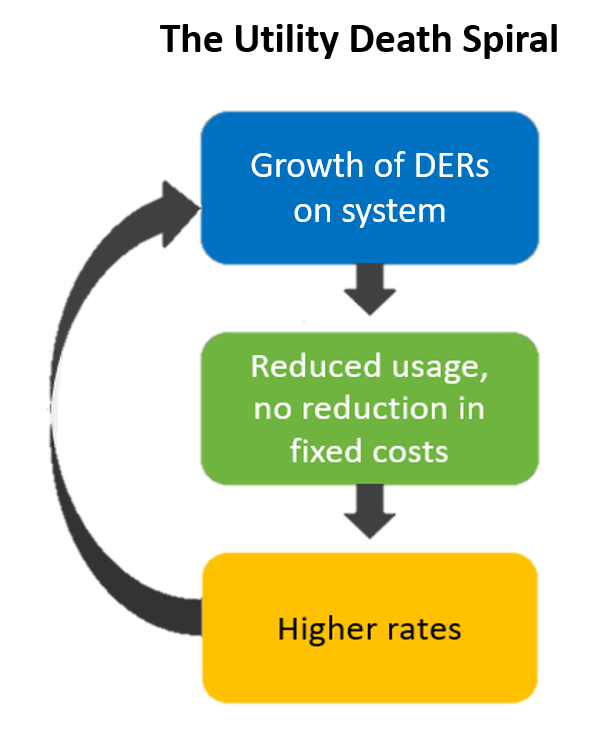
\includegraphics[width=4m]{UtilityDeathSpiral.png}
\caption[Representation of the utility death spiral]{Representation of the utility death spiral \cite{spiral}}
\label{Figure:spiral}
\end{figure}
There are different trends that have been causing the debate surrounding the utility death spiral, as was discussed by Graffy and Kihm \cite{spiralcauses}. Since the emergence of PV adoption is the main cause for the utility death spiral discussion, the reasons for this discussion are the same as the ones that caused PV to become a popular energy technology. As has been discussed in section \ref{Trends}, the main reasons for this are environmental (less GHG emission), technical (less central production, less risk for complete outages \& less stress on grid) and economic (subsidies \& decreasing prices PV technology).
\noindent
One of the reasons why this death spiral is happening, is due to the costs of the electricity transmission and distribution infrastructure being fixed, whereas the fees to the customer are often volumetric, i.e. they are a function of the end consumer's demand \cite{spiral2}. There has been research into the extent to which the utility death spiral has already been manifesting itself \cite{spiral3}. In this research, the effects of PV adoption on the revenues of the utility provider is limited since there is ample non-residential (commercial) demand which, combined with the declining residential demand, will cause the consequences for the TSO/DSO to be limited. Another finding from the research is that the transition to the large PV adoption state will be a smooth one rather than an abrupt one. Darghouth et al. studied how different electricity infrastructure rates influence the feedback on PV deployment \cite{fixedvar}. Since both fixed and time-varying rates will exist in the electricity market, different feedback loops will balance the equilibrium of this market. The fixed tariff will include a positive feedback
\newline \newline \noindent
Despite that there are some signals to confirm the utility death spiral is a consequence of PV adoption, there also voices who suggest that this is due to the traditional tarifing structure of the utilities \cite{spiral4}. Since DERs owners still rely on the distribution infrastructure, not only as consumer but also as producers, a redesign of the distribution tariffs will need to happen. This solution, along with others, will be discussed in the next subsection. A possible way to redesign the tariff structure, as has been proposed in the discussed literature, is by splitting up the fixed and variable costs the grid operator has to incurr and charge the end customer accordingly (based on the grid usage and electricity consumption). This way, DERs production and consumption can be rewarded more efficiently. 
\subsection{Possible solutions}
A possible way to redesign the tariff structure, and thereby mitigate the utility death spiral, as has been proposed in the discussed literature, is by splitting up the fixed and variable costs the grid operator has to incur and charge the end customer accordingly (based on the grid usage and electricity consumption). This way, DERs production and consumption can be rewarded more efficiently \cite{spiral4}. 
\newline \newline \noindent
There are three other ways utilities are exploring to mitigate the potential effects of the utility death spiral, according to an article by Forbes \cite{solutions}. The first one, which is in line with the aforementioned solution, is a transformation of the business model. In doing so, utility providers will focus on ways to exploit the interaction between connected devices on the grid. In doing so, the most valuable locations for DER can be located, allowing for utility providers to adapt their services and pricing in these location to be in a better competitive position, rather than having a uniform electricity charge over the entire grid. In addition, increases in energy efficiency and the use of smart grid are to be compensated by the DERs prosumers. A second avenue that is being considered involves the emergence of EVs. This trend will increase electrification and, therefore, the amount of electricity and ancillary services required on the grid. Utility providers could capitalize on this new trend by offering charging services to the owners of these EVs, either by renting the infrastructure or renting subscriptions to intelligent charging platforms. A final way to combat the utility death spiral is modernizing the grid. To make this costly investment worthwhile for the utility providers, however, utility providers should focus on reducing pollution levels, reducing the average costs of the grid (by increasing the efficiency), increasing customer interaction and improving the grid reliability/resilience. In doing so, the intrinsic value of the grid can be enhanced, creating new opportunities for the utility provider.
\newline \newline \noindent
Although the emergence of DERs, PV in particular, is threatening the current state of affairs for utility providers, there are ample opportunities for these organisations to transform their business model and be prepared for the future. 
\section{Contribution to literature}
Whereas in previous work the adoption of DERs was studied using economically rational theories, like utility maximization or NPV, this Thesis attempts to capture the human character traits in investment decision making. Using cumulative prospect theory (CPT), the subjective perception of the economic utility is used as decision variable, rather than the NPV itself. By incorporating this subjective value, the behavioral traits of individuals, like loss aversion and the reference point of the decision maker will be accounted for. 
\newline \newline \noindent
In addition, this Thesis is one of the only works to study the relationship between DERs adoption on a residential level and the DSO revenues using an ABM. The work that has been done in this domain so far, however, assumed rational behavior by agents \cite{Regulation}. In this work, the adoption of DERs and evolution of network charges are evaluated for different energy-related policies. In doing so, however, the authors assume rational behavior by the electricity consumers. Behavioral traits like risk aversion are not considered in this work. The second major contribution of this Thesis, therefore, is the incorporation of behavioral decision making character traits in the interaction between DER adoption and network charges using
an agent-based modeling framework.